\documentclass{article}

\usepackage{fontspec}
\usepackage{fullpage}
\usepackage{multicol}
\usepackage{multirow}
\usepackage{tikz}

\begin{document}

\newfontfamily\swfill{SuttonSignWritingFill.ttf}
\newfontfamily\swline{SuttonSignWritingLine.ttf}
\newcommand{\bul}{\hfil$\bullet$&}
\renewenvironment{glossary}{\begin{multicols}{5}\begin{center}}{\end{center}\end{multicols}}
\setcounter{secnumdepth}{0}
\setlength{\columnseprule}{1pt}

\section{Supplement For Lesson 8}

\begin{center}
\it
Objectives inspired by, vocabulary transcribed from, and sentences and story by Bill Vicars.

Handshape photos by Adam Frost.

No endorsement implied nor given by either.
\end{center}

\subsection{Objectives}

\begin{tabular}{p{1cm}p{14cm}}
\bul I have completed the objectives for this lesson.\\
\bul I am able to read the numbers 1,000,000 and up.\\
\bul I understand how classifiers are written in SignWriting.\\
\bul I am able demonstrate the meaning and form of the symbol group in the punctuation category.\\
\bul I know which base symbols are in Symbol Groups floor and curve wall.\\
\bul I am able to draw the flat heel palmshape in all forms.\\
\bul I am able to read, write, and sign two thirds of the ASL handshapes in symbol group five.\\
\bul I am able to recognize the vocabulary for this lesson.\\
\bul I am able to read the practice sentences for this lesson.\\
\bul I am able to read the practice story for this lesson.\\
\end{tabular}

\subsection{The Numbers 1,000,000 and Up}

Everything said about the numbers from 1,000 through 999,999 goes at least double if not triple for here.
Expect to see individual digits in almost all writing, but make sure to speak it correctly.

\begin{center}
\begin{tabular}{*{5}{c}}
\textbf{1,000,000}&\textbf{2,000,000}&\textbf{3,000,000}&\textbf{4,000,000}&\textbf{5,000,000}\\
B529x539S20602487x514S15a38500x512S18051504x514S10020511x462S22a04512x496&
B529x539S20602487x514S15a38500x512S18051504x514S10e20511x462S22a04512x496&
B529x539S20602487x514S15a38500x512S18051504x514S11e20502x462S22a04512x496&
B530x539S20602485x514S15a38498x512S18051502x514S14420508x462S22a04510x496&
B529x539S20602486x514S15a38499x512S18051503x514S14c20506x462S22a04511x496\\
\textbf{6,0000,000}&\textbf{7,000,000}&\textbf{8,000,000}&\textbf{9,000,000}\\
B529x539S20602487x514S15a38500x512S18051504x514S18720509x462S22a04512x496&
B530x539S20602486x514S15a38499x512S18051503x514S1a520509x462S22a04511x496&
B530x539S20602486x514S15a38499x512S18051503x514S1bb20509x462S22a04511x496&
B530x539S20602485x514S15a38498x512S18051502x514S1ce20508x462S22a04510x496\\
\end{tabular}
\end{center}

\subsection{Classifiers and SignWriting}

Classifiers follow the same rules as everything else in SignWriting.
Make sure the handshapes, movement, position, and other non-manual markers are correctly transcribed.
You don't need to find the exact handshapes and movements, just the ones that let the classifier be understood.

If you take a look at the story in the last lesson and look at the classifier that specifies the size of the pizza, you will notice that I included a head but did not place any facial expression there.
The reason for that was to (hopefully) correctly specify the size of the pizza, the down arrow and the tense symbol were because every time I signed it I found myself doing a quick down movement and hold to ``set'' the pizza down on an imaginary table in front of me.
The important point isn't to get absolutely everything that you are doing but to get the important stuff that makes it look like a classifier.
The head was definitely important to show that I am showing a pizza larger than my head, perhaps the movement wasn't but I felt that setting the pizza in front of my was important.
But my actual signing was more of a sharply curved fingers and thumbs rather than bent, but I still used the bent L handshapes because I felt that anyone looking at my fingers quickly would interpret it as the standard handshape bent Ls.

\subsection{The Punctuation Category}

The final category has an official name of ``Punctuation'' and only has one base symbol in it.

\begin{center}
\begin{tabular}{ccc}
\textbf{Symbol}\\
\textbf{Group}&\textbf{Name}&\textbf{Example}\\
\textbf{30}&Punctuation&B537x504S38700463x496\\
\end{tabular}
\end{center}

\subsection{Symbol Groups Floor and Curve Wall}

The fifteenth Symbol Group we informally call floor, though it's official name is ``Straight Floor Plane''.
Symbol Group Straight Floor Plane (Floor) has all types of horizontal movement --- back and forth though left and right movement can also be shown.
Each of these arrows have a single tail, to remind us of lines on a road directing you horizontally.

\begin{center}
\begin{tabular}{rcrc}
\textbf{Base Symbol}&\textbf{Example}&\textbf{Base Symbol}&\textbf{Example}\\
Single Straight Movement, Floor Plane Small&B507x508S26500493x493&Single Straight Movement, Floor Plane Medium &B508x515S26600492x485\\
Single Straight Movement, Floor Plane Large&B508x521S26700492x479&Single Straight Movement, Floor Plane Largest&B508x525S26800492x475\\
Single Wrist Flex, Floor Plane             &B508x509S26900492x491&Double Straight Movement, Floor Plane        &B514x507S26a00487x493\\
Double Wrist Flex, Floor Plane             &B514x509S26b00487x491&Double Alternating Movement, Floor Plane     &B514x508S26c00487x493\\
Double Alternating Wrist Flex, Floor Plane &B514x510S26d00487x491&Cross Movement, Floor Plane                  &B516x514S26e00485x487\\
Triple Straight Movement, Floor Plane      &B520x507S26f00480x493&Triple Wrist Flex, Floor Plane               &B520x509S27000480x491\\
Triple Alternating Movement, Floor Plane   &B520x508S27100480x493&Triple Alternating Wrist Flex, Floor Plane   &B520x510S27200480x491\\
Bend, Floor Plane                          &B508x514S27300492x487&Corner, Floor Plane Small                    &B509x509S27400491x492\\
Corner, Floor Plane Medium                 &B512x512S27500488x488&Corner, Floor Plane Large                    &B515x514S27600486x486\\
Check, Floor Plane                         &B510x513S27700490x488&Box, Floor Plane Small                       &B510x509S27800491x491\\
Box, Floor Plane Medium                    &B512x512S27900488x488&Box, Floor Plane Large                       &B515x514S27a00486x486\\
Zigzag, Floor Plane Small                  &B508x513S27b00492x487&Zigzag, Floor Plane Medium                   &B511x517S27c00490x483\\
Zigzag, Floor Plane Large                  &B511x520S27d00489x480&Peaks, Floor Plane Small                     &B512x513S27e00489x488\\
Peaks, Floor Plane Medium                  &B517x518S27f00484x482&Peaks, Floor Plane Large                     &B518x520S28000483x480\\
Travel Rotation Single Floor Plane         &B510x515S28100490x486&Travel Rotation Double Floor Plane           &B510x516S28200490x485\\
Travel Rotation Alternating Floor Plane    &B511x516S28300489x484&Travel Rotation Single Wall Plane            &B511x514S28400489x486\\
Travel Rotation Double Wall Plane          &B511x520S28500489x481&Travel Rotation Alternating Wall Plane       &B513x520S28600488x481\\
Travel Shaking Floor Plane                 &B508x516S28700492x484\\
\end{tabular}
\end{center}

The sixteenth Symbol Group we informally call curve wall, though it's official name is ``Curves Parallel Wall Plane''.
Symbol Group Curves Parallel Wall Plane (Curve Wall) has different types of vertical movement with both up and down as well as left and right movement.

\begin{center}
\begin{tabular}{rcrc}
\textbf{Base Symbol}&\textbf{Example}&\textbf{Base Symbol}&\textbf{Example}\\
Curve Wall Plane, Quarter Small         &B506x511S28800494x489&Curve Wall Plane, Quarter Medium         &B508x515S28900493x486\\
Curve Wall Plane, Quarter Large         &B509x518S28a00492x482&Curve Wall Plane, Quarter Largest        &B510x522S28b00490x478\\
Curve Wall Plane, Half Circle Small     &B511x514S28c00490x486&Curve Wall Plane, Half Circle Medium     &B512x517S28d00488x484\\
Curve Wall Plane, Half Circle Large     &B515x518S28e00486x482&Curve Wall Plane, Half Circle Largest    &B519x527S28f00482x473\\
Curve Wall Plane, 3 Quarter Circle Small&B512x514S29000489x487&Curve Wall Plane, 3 Quarter Circle Medium&B514x517S29100486x484\\
Hump Wall Plane Small                   &B507x516S29200493x485&Hump Wall Plane Medium                   &B507x521S29300493x480\\
Hump Wall Plane Large                   &B508x522S29400492x478&Loop Wall Plane Small                    &B507x516S29500494x485\\
Loop Wall Plane Medium                  &B508x517S29600493x483&Loop Wall Plane Large                    &B510x524S29700491x477\\
Loop Wall Plane Small Double            &B507x522S29800494x478&Wave Wall Plane 2 Curves Small           &B507x516S29900493x484\\
Wave Wall Plane 2 Curves Medium         &B508x518S29a00493x483&Wave Wall Plane 2 Curves Large           &B509x520S29b00491x481\\
Wave Wall Plane 3 Curves Small          &B509x519S29c00492x482&Wave Wall Plane 3 Curves Medium          &B511x526S29d00490x475\\
Wave Wall Plane 3 Curves Large          &B515x526S29e00485x475&Curve Then Straight Movement Wall Plane  &B510x517S29f00491x484\\
Curved Cross Movement Wall Small        &B511x513S2a000490x487&Curved Cross Movement Wall Medium        &B514x517S2a100487x483\\
Rotation Single Wall Plane              &B512x514S2a200489x486&Rotation Double Wall Plane               &B512x518S2a300489x482\\
Rotation Alternate Wall Plane           &B513x518S2a400488x482&Shaking Wall Plane                       &B511x517S2a500490x484\\
\end{tabular}
\end{center}

Before you can consider this lesson complete, you need to be able to list off the symbol groups as:
``one, two, three, four, five, six, seven, eight, nine, thumb;''
``contact, finger, wall, diagonal, floor, curve wall.''

Some additional help when remembering the second set of base symbols.

We had wall to complete the next portion of the second set, and we started back with wall.
This should not be surprising since wall is first.

\subsection{The Flat Heel Palmshape}

Like with the Fist Heel Palmshape, the Flat Heel Palmshape only comes as fill 2 and means palm up in the primary rotation.

\begin{center}
\begin{tabular}{r*{6}{c}}
&\textbf{Fill 1}&\textbf{Fill 2}&\textbf{Fill 3}&\textbf{Fill 4}&\textbf{Fill 5}\textbf{Fill 6}\\
\textbf{Right}&---&B510x505S15c10490x496&---&---&---&---\\
\textbf{Left} &---&B510x505S15c18490x496&---&---&---&---\\
\end{tabular}
\end{center}

\subsection{More ASL Handshapes From Symbol Group Five}

The twenty one handshapes in Symbol Group Five used by ASL in order are:
Five Fingers Spread;
Five Fingers Spread Heel;
Five Fingers Spread, Four Bent;
Five Fingers Spread, Four Bent Heel;
Five Fingers Spread Bent;
Five Fingers Spread Bent Heel;
Five Fingers Spread Cup;
{\it
Five Fingers Spread Cup Open;
Five Fingers Spread Hinge;
Flat Hand;
Flat Heel;
Flat, Thumb Side;
Flat, Thumb Side Heel;
Cup;
}
Cup, Thumb Side;
Cup, No Thumb;
Circle;
Hinge;
Hinge, Thumb Side
Hinge, No Thumb
and Angle.

\subsubsection{The Five Fingers Spread Cup Open handshape}

\begin{center}
\begin{tabular}{r*{6}{c}}
&\textbf{Fill 1}&\textbf{Fill 2}&\textbf{Fill 3}&\textbf{Fill 4}&\textbf{Fill 5}&\textbf{Fill 6}\\
\multirow{2}{*}{\textbf{Right}}&
B508x513S15400493x488&
B508x513S15410493x488&
B508x513S15420493x488&
B508x513S15430493x488&
B508x513S15440493x488&
B508x513S15450493x488\\
&
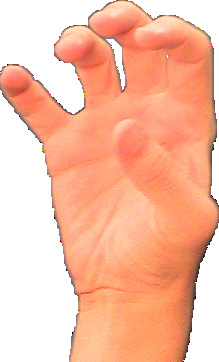
\includegraphics[scale=0.1]{images/05-08-1.jpg}&
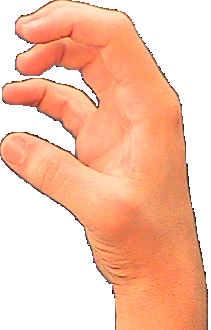
\includegraphics[scale=0.1]{images/05-08-2.jpg}&
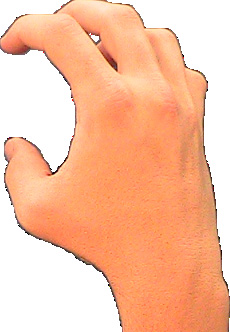
\includegraphics[scale=0.1]{images/05-08-3.jpg}&
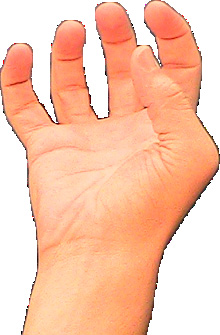
\includegraphics[scale=0.1]{images/05-08-4.jpg}&
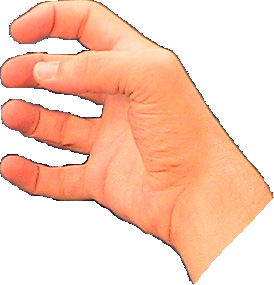
\includegraphics[scale=0.1]{images/05-08-5.jpg}&
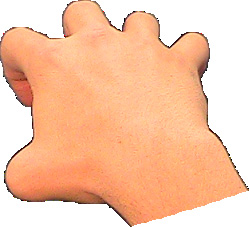
\includegraphics[scale=0.1]{images/05-08-6.jpg}\\
\textbf{Left}&
B508x513S15408493x488&
B508x513S15418493x488&
B508x513S15428493x488&
B508x513S15438493x488&
B508x513S15448493x488&
B508x513S15458493x488\\
\end{tabular}
\end{center}

\subsubsection{The Five Fingers Spread Hinge handshape}

\begin{center}
\begin{tabular}{r*{6}{c}}
&\textbf{Fill 1}&\textbf{Fill 2}&\textbf{Fill 3}&\textbf{Fill 4}&\textbf{Fill 5}&\textbf{Fill 6}\\
\multirow{2}{*}{\textbf{Right}}&
B509x513S15700491x487&
B509x513S15710491x487&
B509x513S15720491x487&
B509x513S15730491x487&
B509x513S15740491x487&
B509x513S15750491x487\\
&
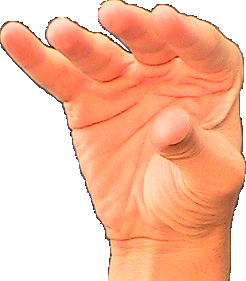
\includegraphics[scale=0.1]{images/05-09-1.jpg}&
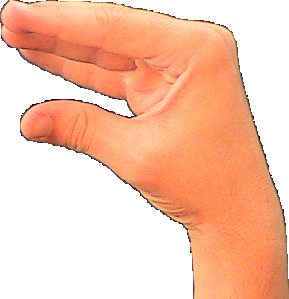
\includegraphics[scale=0.1]{images/05-09-2.jpg}&
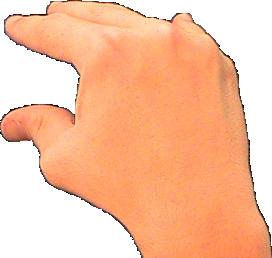
\includegraphics[scale=0.1]{images/05-09-3.jpg}&
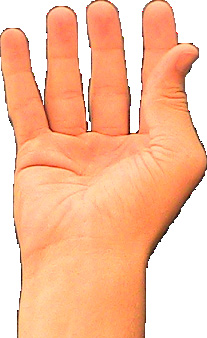
\includegraphics[scale=0.1]{images/05-09-4.jpg}&
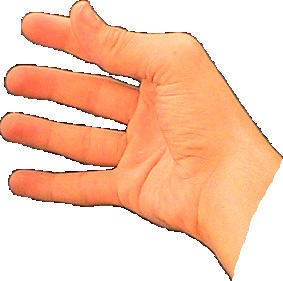
\includegraphics[scale=0.1]{images/05-09-5.jpg}&
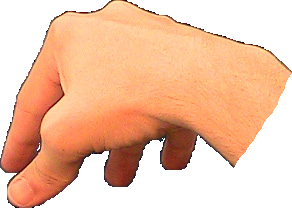
\includegraphics[scale=0.1]{images/05-09-6.jpg}\\
\textbf{Left}&
B509x513S15708491x487&
B509x513S15718491x487&
B509x513S15728491x487&
B509x513S15738491x487&
B509x513S15748491x487&
B509x513S15758491x487\\
\end{tabular}
\end{center}

Writing fills 3 and 6 might confuse you at first.
Remember when we talked about using a circle to indicate the finger pointing at the signer we also mentioned that you could write it using a symbol that looked like the second fill.
When writing this symbol, you should do that unless you are spending time to ``paint'' handshapes.
And note that the thumb would go on the opposite side of fill 2 for fills 1 and 4.

\subsubsection{The Flat Hand handshape}

\begin{center}
\begin{tabular}{r*{6}{c}}
&\textbf{Fill 1}&\textbf{Fill 2}&\textbf{Fill 3}&\textbf{Fill 4}&\textbf{Fill 5}&\textbf{Fill 6}\\
\multirow{2}{*}{\textbf{Right}}&
B506x514S15a00494x487&
B506x514S15a10494x487&
B506x514S15a20494x487&
B506x514S15a30494x487&
B506x514S15a40494x487&
B506x514S15a50494x487\\
&
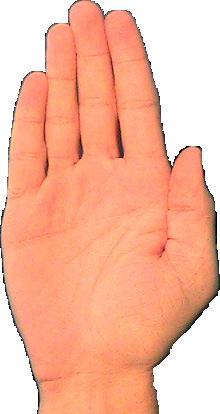
\includegraphics[scale=0.1]{images/05-10-1.jpg}&
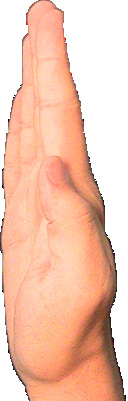
\includegraphics[scale=0.1]{images/05-10-2.jpg}&
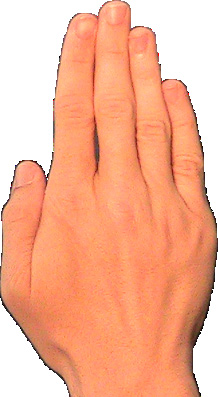
\includegraphics[scale=0.1]{images/05-10-3.jpg}&
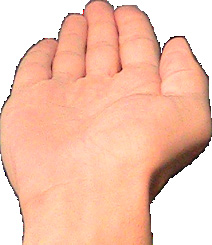
\includegraphics[scale=0.1]{images/05-10-4.jpg}&
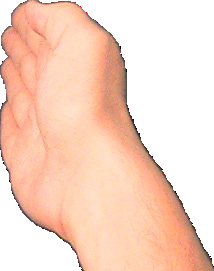
\includegraphics[scale=0.1]{images/05-10-5.jpg}&
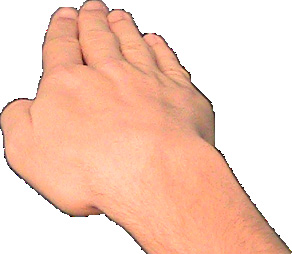
\includegraphics[scale=0.1]{images/05-10-6.jpg}\\
\textbf{Left}&
B506x514S15a08494x487&
B506x514S15a18494x487&
B506x514S15a28494x487&
B506x514S15a38494x487&
B506x514S15a48494x487&
B506x514S15a58494x487\\
\end{tabular}
\end{center}

\subsubsection{The Flat Heel handshape}

\begin{center}
\begin{tabular}{r*{6}{c}}
&\textbf{Fill 1}&\textbf{Fill 2}&\textbf{Fill 3}&\textbf{Fill 4}&\textbf{Fill 5}&\textbf{Fill 6}\\
\multirow{2}{*}{\textbf{Right}}&
\multirow{2}{*}{---}&
B510x505S15c10490x496&
\multirow{2}{*}{---}&
\multirow{2}{*}{---}&
\multirow{2}{*}{---}&
\multirow{2}{*}{---}\\
&
&
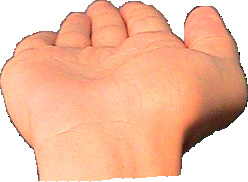
\includegraphics[scale=0.1]{images/05-11-2.jpg}\\
\textbf{Left}&
---&
B510x505S15c18490x496&
---&
---&
---&
---\\
\end{tabular}
\end{center}

\subsubsection{The Flat, Thumb Side handshape}

\begin{center}
\begin{tabular}{r*{6}{c}}
&\textbf{Fill 1}&\textbf{Fill 2}&\textbf{Fill 3}&\textbf{Fill 4}&\textbf{Fill 5}&\textbf{Fill 6}\\
\multirow{2}{*}{\textbf{Right}}&
B510x514S15d00491x487&
B510x514S15d10491x487&
B510x514S15d20491x487&
B510x514S15d30491x487&
B510x514S15d40491x487&
B510x514S15d50491x487\\
&
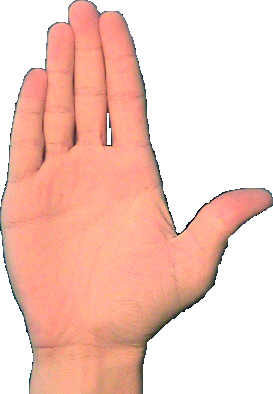
\includegraphics[scale=0.1]{images/05-12-1.jpg}&
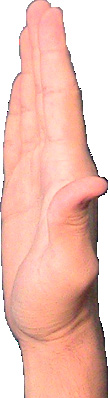
\includegraphics[scale=0.1]{images/05-12-2.jpg}&
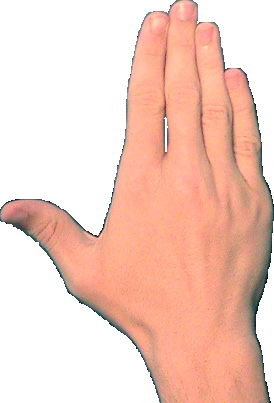
\includegraphics[scale=0.1]{images/05-12-3.jpg}&
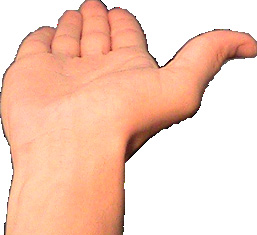
\includegraphics[scale=0.1]{images/05-12-4.jpg}&
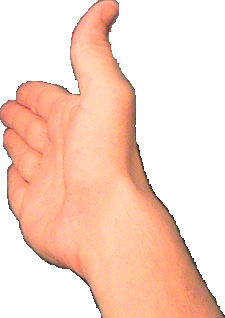
\includegraphics[scale=0.1]{images/05-12-5.jpg}&
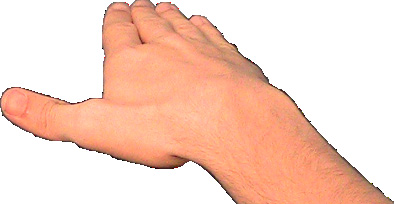
\includegraphics[scale=0.1]{images/05-12-6.jpg}\\
\textbf{Left}&
B510x514S15d08491x487&
B510x514S15d18491x487&
B510x514S15d28491x487&
B510x514S15d38491x487&
B510x514S15d48491x487&
B510x514S15d58491x487\\
\end{tabular}
\end{center}

\subsubsection{The Flat, Thumb Side Heel handshape}

\begin{center}
\begin{tabular}{r*{6}{c}}
&\textbf{Fill 1}&\textbf{Fill 2}&\textbf{Fill 3}&\textbf{Fill 4}&\textbf{Fill 5}&\textbf{Fill 6}\\
\multirow{2}{*}{\textbf{Right}}&
\multirow{2}{*}{---}&
B514x505S15e10487x495&
\multirow{2}{*}{---}&
\multirow{2}{*}{---}&
\multirow{2}{*}{---}&
\multirow{2}{*}{---}\\
&
&
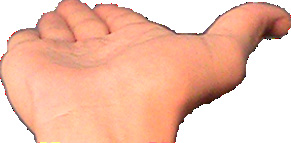
\includegraphics[scale=0.1]{images/05-13-2.jpg}\\
\textbf{Left}&
---&
B514x505S15e18487x495&
---&
---&
---&
---\\
\end{tabular}
\end{center}

\subsubsection{The Cup Handshape}

\begin{center}
\begin{tabular}{r*{6}{c}}
&\textbf{Fill 1}&\textbf{Fill 2}&\textbf{Fill 3}&\textbf{Fill 4}&\textbf{Fill 5}&\textbf{Fill 6}\\
\multirow{2}{*}{\textbf{Right}}&
B509x510S16d00492x490&
B509x510S16d10492x490&
B509x510S16d20492x490&
B509x510S16d30492x490&
B509x510S16d40492x490&
B509x510S16d50492x490\\
&
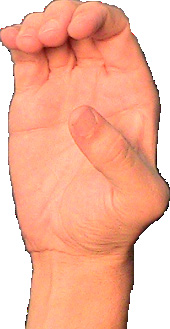
\includegraphics[scale=0.1]{images/05-14-1.jpg}&
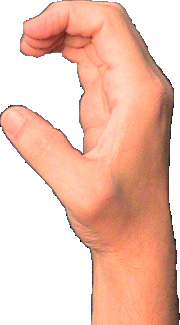
\includegraphics[scale=0.1]{images/05-14-2.jpg}&
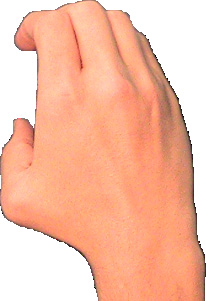
\includegraphics[scale=0.1]{images/05-14-3.jpg}&
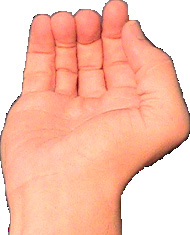
\includegraphics[scale=0.1]{images/05-14-4.jpg}&
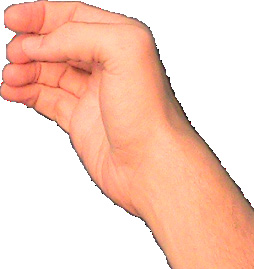
\includegraphics[scale=0.1]{images/05-14-5.jpg}&
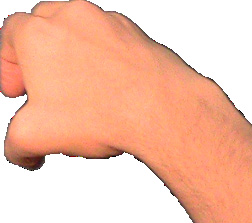
\includegraphics[scale=0.1]{images/05-14-6.jpg}\\
\textbf{Left}&
B509x510S16d08492x490&
B509x510S16d18492x490&
B509x510S16d28492x490&
B509x510S16d38492x490&
B509x510S16d48492x490&
B509x510S16d58492x490\\
\end{tabular}
\end{center}

\subsection{Vocabulary}

\begin{glossary}

\textbf{1,000,000}\\
AS10020S22a04S18051S15a38S20602M529x539S20602487x514S15a38500x512S18051504x514S10020511x462S22a04512x496

\textbf{2,000,000}\\
AS10e20S22a04S18051S15a38S20602M529x539S20602487x514S15a38500x512S18051504x514S10e20511x462S22a04512x496

\textbf{3,000,000}\\
AS11e20S22a04S18051S15a38S20602M529x539S20602487x514S15a38500x512S18051504x514S11e20502x462S22a04512x496

\textbf{4,000,000}\\
AS14420S22a04S18051S15a38S20602M530x539S20602485x514S15a38498x512S18051502x514S14420508x462S22a04510x496

\textbf{5,000,000}\\
AS14c20S22a04S18051S15a38S20602M529x539S20602486x514S15a38499x512S18051503x514S14c20506x462S22a04511x496

\textbf{6,000,000}\\
AS18720S22a04S18051S15a38S20602M529x539S20602487x514S15a38500x512S18051504x514S18720509x462S22a04512x496

\textbf{7,000,000}\\
AS1a520S22a04S18051S15a38S20602M530x539S20602486x514S15a38499x512S18051503x514S1a520509x462S22a04511x496

\textbf{8,000,000}\\
AS1bb20S22a04S18051S15a38S20602M530x539S20602486x514S15a38499x512S18051503x514S1bb20509x462S22a04511x496

\textbf{9,000,000}\\
AS1ce20S22a04S18051S15a38S20602M530x539S20602485x514S15a38498x512S18051502x514S1ce20508x462S22a04510x496

\textbf{adapt}\\
AS10621S10609S21100S2df20M522x534S10609499x502S10621479x514S21100491x493S2df20487x467

\textbf{backpack}\\
AS1f702S1f70aS20600S20600S2fb04S36e00M536x525S36e00477x476S1f702516x487S1f70a467x487S20600514x510S20600463x510S2fb04493x519

\textbf{basket}\\
AS15406S1540eS28907S2891fS2fb00M537x524S15406503x509S1540e475x508S28a07507x477S28a1f464x477S2fb00494x486

\textbf{battery}\\
AS10642S1064aS26a02S26a16S20602M533x525S10642507x510S1064a468x509S26a02507x476S26a16482x475S20602495x487

\textbf{belt}\\
AS11502S1150aS2d600S2d618S36d00S36d00M532x524S1150a468x503S11502501x503S2d600503x488S36d00479x520S36d00479x476S2d618469x488

\textbf{change}\\
AS10621S10609S21100S2df20M522x534S10609499x502S10621479x514S21100491x493S2df20487x467

\textbf{clothes}\\
AS14c03S14c0bS20e00S2c601S2c601S20e00S2c610S2c610M569x521S20e00473x509S20e00516x509S14c0b462x479S14c03510x480S2c601533x494S2c610449x494S2c601550x494S2c610432x494

\textbf{coat}\\
AS1f701S1f709S21100S28804S2881cS2fb04S36d00M528x532S36d00479x469S1f701507x479S1f709471x479S28804511x503S2881c476x503S21100494x507S2fb04492x526

\textbf{convert}\\
AS10621S10609S21100S2df20M522x534S10609499x502S10621479x514S21100491x493S2df20487x467

\textbf{dirty}\\
AS14c52S22512S2ff00M518x541S22512467x515S2ff00482x483S14c52481x517

\textbf{dress}\\
AS14c03S14c0bS20e00S2c601S20e00S2c610M552x521S20e00473x509S20e00516x509S14c0b462x479S14c03510x480S2c601533x494S2c610449x494

\textbf{electricity}\\
AS10642S1064aS26a02S26a16S20602M533x525S10642507x510S1064a468x509S26a02507x476S26a16482x475S20602495x487

\textbf{Gallaudet}\\
AS1dc21S26506S1f410S31410M580x518S31410482x483S1dc21511x483S1f410551x489S26506541x494

\textbf{glasses}\\
AS1dc21S26506S1f410S31410M580x518S31410482x483S1dc21511x483S1f410551x489S26506541x494

\textbf{hearing aid}\\
AS10611S20600S2ff00M543x525S2ff00482x483S10611520x497S20600520x482

\textbf{jacket}\\
AS1f701S1f709S21100S28804S2881cS2fb04S36d00M528x532S36d00479x469S1f701507x479S1f709471x479S28804511x503S2881c476x503S21100494x507S2fb04492x526

\textbf{million}\\
AS18051S15a38S20602M521x514S20602479x489S15a38492x487S18051496x489

\textbf{off}\\
AS17620S1ce20S26706M532x524S17620469x490S1ce20488x476S26706490x508

\textbf{on}\\
AS15a51S15a57S20500M518x522S15a57482x479S15a51495x499S20500503x488

\textbf{pants}\\
AS18003S1800bS20e00S20e00S22f00S22f10S36d10M548x531S1800b517x506S18003465x506S22f00523x474S22f10450x474S20e00530x491S20e00457x491S36d10479x470

\textbf{pick-up}\\
AS1d150S1ce50S22a00M515x542S1d150485x514S1ce50493x458S22a00492x493

\textbf{shirt}\\
AS1d411S26a00S20800S36d00M562x530S20800515x520S26a00535x485S36d00479x471S1d411507x491

\textbf{shoes}\\
AS20350S20350S20600M516x515S20350484x500S20350501x500S20600489x486

\textbf{socks}\\
AS10004S1000cS21100S23100S23118M539x529S10004506x499S23100513x480S1000c479x499S23118461x480S21100494x480S2fb00492x471

\textbf{underwear}\\
AS1dc04S1dc0cS2d604S2d61cS2fb00S18504S1850cS36d00S36d00M593x527S36d00479x474S36d00480x507S1dc04521x485S1dc0c454x485S2d604541x502S2d61c432x502S18504569x483S1850c408x485S2fb00494x521

\textbf{washing machine}\\
AS15411S1541fS2c500S2c514M561x526S15411493x474S1541f484x493S2c500521x479S2c514440x501

\textbf{which}\\
AS1f502S1f502S23100S23110S2fb04M535x526S2fb04491x520S1f502512x474S23100509x503S23110465x505S1f502471x474

\textbf{zip}\\
AS1f420S10e08S22b00S21100S11508M525x544S1f420496x528S21100476x495S22b00490x494S10e08479x514S11508476x456

\end{glossary}

\subsection{Practice Sheet 8.A}

\begin{multicols}{5}
\begin{center}

M508x515S10000493x485 % 1
\\M536x504S38800464x496 % .
\\M536x525S36e00477x476S1f702516x487S1f70a467x487S20600514x510S20600463x510S2fb04493x519 % backpack
\\M537x504S38700463x496 % ,
\\M518x518S30a00482x483 % y/n
\\M510x523S10040495x493S26500491x478 % you
\\M532x518S18049468x483S18041507x483S20500486x507S20500504x507 % have
\\M536x507S38900464x493 % ?
\vfil
\columnbreak

M508x515S10e00493x485 % 2
\\M536x504S38800464x496 % .
\\M507x523S15a28494x496S26500493x477 % your
\\M525x539S15a11502x476S15a19476x476S20500495x462S23904505x501S2391c477x501S2fb04494x533 % house
\\M537x504S38700463x496 % ,
\\M569x521S20e00473x509S20e00516x509S14c0b462x479S14c03510x480S2c601533x494S2c610449x494S2c601550x494S2c610432x494 % clothes
\\M518x541S22512467x515S2ff00482x483S14c52481x517 % dirty
\\M537x504S38700463x496 % ,
\\M518x518S30c00482x483 % \?
\\M522x531S2b720489x469S18527503x504S1852f479x503 % put (in)
\\M537x524S15406503x509S1540e475x508S28a07507x477S28a1f464x477S2fb00494x486 % basket
\\M518x540S34600482x483S1e111473x512S21800463x502 % who
\\M536x507S38900464x493 % ?
\vfil
\columnbreak

M512x515S11e00489x485 % 3
\\M536x504S38800464x496 % .
\\M507x523S15a28494x496S26500493x477 % your
\\M543x525S2ff00482x483S10611520x497S20600520x482 % hearing aid
\\M537x504S38700463x496 % ,
\\M533x525S10642507x510S1064a468x509S26a02507x476S26a16482x475S20602495x487 % battery
\\M537x504S38700463x496 % ,
\\M518x518S30c00482x483 % \?
\\M524x532S14249491x508S14240477x480S2e800510x469S20500480x509 % kind
\\M536x507S38900464x493 % ?
\vfil
\columnbreak

M511x516S14400489x485 % 4
\\M536x504S38800464x496 % .
\\M507x523S15a28494x496S26500493x477 % your
\\M532x524S1150a468x503S11502501x503S2d600503x488S36d00479x520S36d00479x476S2d618469x488 % belt
\\M537x504S38700463x496 % ,
\\M518x518S30c00482x483 % \?
\\M518x565S14c00488x534S22520484x520S2ff00482x483 % color
\\M536x507S38900464x493 % ?
\vfil
\columnbreak

M512x516S14c00489x485 % 5
\\M536x504S38800464x496 % .
\\M510x523S10040495x493S26500491x478 % you
\\M522x534S10609499x502S10621479x514S21100491x493S2df20487x467 % change
\\M569x521S20e00473x509S20e00516x509S14c0b462x479S14c03510x480S2c601533x494S2c610449x494S2c601550x494S2c610432x494 % clothes
\\M537x504S38700463x496 % ,
\\M518x518S30c00482x483 % \?
\\M536x522S10019464x492S10012487x492S2e708521x486S20500476x478 % when
\\M536x507S38900464x493 % ?
\vfil

\end{center}
\end{multicols}

\subsection{Practice Sheet 8.B}

\begin{multicols}{5}
\begin{center}

M509x515S18720491x486 % 6
\\M536x504S38800464x496 % .
\\M527x518S15a39497x482S18020497x503S20600473x498 % doctor
\\M512x515S1dc20488x485 % l
\\M510x508S1f720490x493 % a
\\M507x511S14720493x489 % b
\\M528x532S36d00479x469S1f701507x479S1f709471x479S28804511x503S2881c476x503S21100494x507S2fb04492x526 % coat
\\M537x504S38700463x496 % ,
\\M518x518S30c00482x483 % \?
\\M518x565S14c00488x534S22520484x520S2ff00482x483 % color
\\M536x507S38900464x493 % ?
\vfil
\columnbreak

M511x514S1a520490x486 % 7
\\M536x504S38800464x496 % .
\\M569x521S20e00473x509S20e00516x509S14c0b462x479S14c03510x480S2c601533x494S2c610449x494S2c601550x494S2c610432x494 % clothes
\\M518x541S22512467x515S2ff00482x483S14c52481x517 % dirty
\\M537x504S38700463x496 % ,
\\M518x518S30c00482x483 % \?
\\M514x524S10620486x476S23004489x506 % should
\\M522x531S2b720489x469S18527503x504S1852f479x503 % put
\\M518x525S10020482x476S27106503x485 % where
\\M536x507S38900464x493 % ?
\vfil
\columnbreak

M511x514S1bb20490x486 % 8
\\M536x504S38800464x496 % .
\\M515x519S10047485x498S26507501x481 % 3rd person
\\M538x527S15a40511x475S15a48481x473S22104526x478S22104465x478S18048463x510S18040506x512 % room
\\M532x518S18049468x483S18041507x483S20500486x507S20500504x507 % have
\\M580x518S31410482x483S1dc21511x483S1f410551x489S26506541x494 % glasses
\\M518x518S30c00482x483 % \?
\\M518x540S34600482x483S1e111473x512S21800463x502 % who
\\M536x507S38900464x493 % ?
\vfil
\columnbreak

M511x515S1ce20489x485 % 9
\\M536x504S38800464x496 % .
\\M543x525S2ff00482x483S10611520x497S20600520x482 % hearing aid
\\M537x504S38700463x496 % ,
\\M518x518S30c00482x483 % \?
\\M518x540S34600482x483S1e111473x512S21800463x502 % who
\\M532x518S18049468x483S18041507x483S20500486x507S20500504x507 % have
\\M536x507S38900464x493 % ?
\vfil
\columnbreak

M513x528S2a538494x472S1f540488x504 % 10
\\M536x504S38800464x496 % .
\\M518x518S30a00482x483 % y/n
\\M510x523S10040495x493S26500491x478 % you
\\M516x540S1bb02488x461S14c02484x517S20e00499x502S26500499x483 % like
\\M561x526S15411493x474S1541f484x493S2c500521x479S2c514440x501 % washing machine
\\M569x521S20e00473x509S20e00516x509S14c0b462x479S14c03510x480S2c601533x494S2c610449x494S2c601550x494S2c610432x494 % clothes
\\M536x507S38900464x493 % ?
\vfil

\end{center}
\end{multicols}

\subsection{Practice Sheet 8.C}

\begin{multicols}{5}
\begin{center}

M512x520S10000489x490S21d00494x480 % 11
\\M536x504S38800464x496 % .
\\M563x518S2ff00482x483S19200542x478S26a04519x487S20500504x501 % suppose
\\M510x523S10040495x493S26500491x478 % you
\\M525x526S10018476x477S10018497x496S2882a503x475 % go
\\M523x517S15a56478x505S16d20481x483S20600501x494 % church
\\M537x504S38700463x496 % ,
\\M518x518S30c00482x483 % \?
\\R548x531S1800b517x506S18003465x506S22f00523x474S22f10450x474S20e00530x491S20e00457x491S36d10479x470 % pants
\\L552x521S20e00473x509S20e00516x509S14c0b462x479S14c03510x480S2c601533x494S2c610449x494 % dress
\\M510x523S10040495x493S26500491x478 % you
\\M535x526S2fb04491x520S1f502512x474S23100509x503S23110465x505S1f502471x474 % which
\\M536x507S38900464x493 % ?
\vfil
\columnbreak

M509x521S10e00491x491S21d00491x480 % 12
\\M536x504S38800464x496 % .
\\M548x531S1800b517x506S18003465x506S22f00523x474S22f10450x474S20e00530x491S20e00457x491S36d10479x470 % pants
\\M537x504S38700463x496 % ,
\\M529x523S14c50476x492S22520472x478S26606499x505 % fingerspell
\\M536x504S38800464x496 % .
\vfil
\columnbreak

M513x519S22114487x481S12d00489x489 % 13
\\M536x504S38800464x496 % .
\\M512x519S15a39489x496S15a5f488x496S20600489x482 % school
\\M529x532S14c00506x501S14c08472x501S2df08507x476S2df10472x476S2fb00490x469 % finish
\\M537x504S38700463x496 % ,
\\M507x523S15a28494x496S26500493x477 % your
\\M518x535S2ff00482x483S20500494x520S14c10471x504 % mother
\\M515x542S1d150485x514S1ce50493x458S22a00492x493 % pick up
\\M510x523S10040495x493S26500491x478 % you
\\M537x504S38700463x496 % ,
\\M518x518S30c00482x483 % \?
\\M521x518S10013490x482S15a1a494x506S20500480x505 % time
\\M536x507S38900464x493 % ?
\vfil
\columnbreak

M513x515S14700493x493S22114487x486 % 14
\\M536x504S38800464x496 % .
\\M507x523S15a28494x496S26500493x477 % your
\\M562x530S20800515x520S26a00535x485S36d00479x471S1d411507x491 % shirt
\\M537x504S38700463x496 % ,
\\M518x518S30c00482x483 % \?
\\M518x565S14c00488x534S22520484x520S2ff00482x483 % color
\\M536x507S38900464x493 % ?
\vfil
\columnbreak

M513x518S22114487x483S15d00494x491 % 15
\\M536x504S38800464x496 % .
\\M516x515S20350484x500S20350501x500S20600489x486 % shoes
\\M537x504S38700463x496 % ,
\\M518x518S30c00482x483 % \?
\\M510x523S10040495x493S26500491x478 % you
\\M532x518S18049468x483S18041507x483S20500486x507S20500504x507 % have
\\M526x535S22a20494x501S14c08474x465S14c00503x465S20338478x520S20330508x520 % how many
\\M536x507S38900464x493 % ?
\vfil

\end{center}
\end{multicols}

\subsection{Practice Sheet 8.D}

\begin{multicols}{5}
\begin{center}

M520x522S18700502x492S2e00e480x479 % 16
\\M536x504S38800464x496 % .
\\M507x523S15a28494x496S26500493x477 % your
\\M539x529S10004506x499S23100513x480S1000c479x499S23118461x480S21100494x480S2fb00492x471 % socks
\\M537x504S38700463x496 % ,
\\M518x518S30c00482x483 % \?
\\M518x565S14c00488x534S22520484x520S2ff00482x483 % color
\\M536x507S38900464x493 % ?
\vfil
\columnbreak

M522x522S1a500501x494S2e00e478x478 % 17
\\M536x504S38800464x496 % .
\\M518x518S30a00482x483 % y/n
\\M510x523S10040495x493S26500491x478 % you
\\M539x519S2ff00482x483S10011518x489S20500510x474 % think
\\M522x525S15a50478x475S22a04483x510S2d508500x511 % children
\\M514x524S10620486x476S23004489x506 % should
\\M522x534S10609499x502S10621479x514S21100491x493S2df20487x467 % change
\\M593x527S36d00479x474S36d00480x507S1dc04521x485S1dc0c454x485S2d604541x502S2d61c432x502S18504569x483S1850c408x485S2fb00494x521 % underwear
\\M541x520S26a00514x474S2ff00482x483S20e00521x490S1f710514x505 % daily
\\M536x507S38900464x493 % ?
\vfil
\columnbreak

M523x522S1bb00502x492S2e00e478x479 % 18
\\M536x504S38800464x496 % .
\\R550x522S1f720530x506S11820451x478S2470a482x496 % pizza
\\L515x543S20800505x533S20800486x457S16d21488x471S1710f490x507S17107496x466S16d29492x513 % hamburger
\\M518x518S30c00482x483 % \?
\\M510x523S10040495x493S26500491x478 % you
\\M540x543S1c507499x518S20600518x508S2ff00482x483 % favorite
\\M535x526S2fb04491x520S1f502512x474S23100509x503S23110465x505S1f502471x474 % which
\\M536x507S38900464x493 % ?
\vfil
\columnbreak

M524x522S1ce00502x490S2e00e477x479 % 19
\\M536x504S38800464x496 % .
\\M507x523S15a28494x496S26500493x477 % your
\\M536x525S36e00477x476S1f702516x487S1f70a467x487S20600514x510S20600463x510S2fb04493x519 % backpack
\\M532x518S18049468x483S18041507x483S20500486x507S20500504x507 % have
\\M525x544S1f420496x528S21100476x495S22b00490x494S10e08479x514S11508476x456 % zip
\\M536x507S38900464x493 % ?
\vfil
\columnbreak

M517x513S22114484x488S1f420488x498 % 20
\\M536x504S38800464x496 % .
\\M518x518S30a00482x483 % y/n
\\M510x523S10040495x493S26500491x478 % you
\\M534x543S14c30507x457S14c38469x458S15030508x512S15038467x511S26524493x493 % want
\\M525x526S10018476x477S10018497x496S2882a503x475 % go
\\M580x518S31410482x483S1dc21511x483S1f410551x489S26506541x494 % gallaudet
\\M534x518S2ff00482x483S15a10522x485S2b700513x453 % future
\\M536x507S38900464x493 % ?
\vfil

\end{center}
\end{multicols}

\subsection{Story 8}

\begin{multicols}{5}
\begin{center}
M513x514S15a01490x486S20500487x503 % my
\\M518x535S2ff00482x483S20500494x520S14c10471x504 % mother
\\M561x526S15411493x474S1541f484x493S2c500521x479S2c514440x501 % washing machine
\\M541x520S26a00514x474S2ff00482x483S20e00521x490S1f710514x505 % daily
\\M536x504S38800464x496 % .

M520x546S15a37481x523S1f502485x486S20500488x509S28929493x455 % help (I to 3rd)
\\M536x504S38800464x496 % .

M561x526S15411493x474S1541f484x493S2c500521x479S2c514440x501 % washing machine
\\M518x518S10043488x483S20500482x507 % me
\\R518x530S17d20495x515S21600485x517S25600483x479S18520493x470 % grab and lift lid to open machine
\\M569x521S20e00473x509S20e00516x509S14c0b462x479S14c03510x480S2c601533x494S2c610449x494S2c601550x494S2c610432x494 % clothes
\\M518x541S22512467x515S2ff00482x483S14c52481x517 % dirty
\\L550x532S14c50452x468S18550451x510S26606489x510S14c50526x501 % pick up, move, and drop
\\M536x504S38800464x496 % .

M548x531S1800b517x506S18003465x506S22f00523x474S22f10450x474S20e00530x491S20e00457x491S36d10479x470 % pants
\\M537x504S38700463x496 % ,
\\M562x530S20800515x520S26a00535x485S36d00479x471S1d411507x491 % shirt
\\M537x504S38700463x496 % ,
\\M539x529S10004506x499S23100513x480S1000c479x499S23118461x480S21100494x480S2fb00492x471 % socks
\\M537x504S38700463x496 % ,
\\M593x527S36d00479x474S36d00480x507S1dc04521x485S1dc0c454x485S2d604541x502S2d61c432x502S18504569x483S1850c408x485S2fb00494x521 % underwear
\\M537x504S38700463x496 % ,
\\M550x532S14c50452x468S18550451x510S26606489x510S14c50526x501 % pick up, move, and drop
\\M536x504S38800464x496 % .

M513x514S15a01490x486S20500487x503 % my
\\M543x525S2ff00482x483S10611520x497S20600520x482 % hearing aid
\\M536x507S38900464x493 % ?

M518x518S10043488x483S20500482x507 % me
\\M516x538S1bb02488x517S14c52484x463S2d200490x490 % don't like
\\M536x504S38800464x496 % .

M576x525S2ff00482x483S10611520x497S20600520x482S2d608547x497 % take off hearing aid
\\M537x504S38700463x496 % ,
\\M564x527S2f800481x443S10611541x499S2ff00482x483S2e108490x447 % hold hearing aid while looking both directions
\\M522x531S2b720489x469S18527503x504S1852f479x503 % put
\\M517x537S17d20494x464S21600484x466S18520487x522S25a04483x483 % close washing machine lid
\\M520x560S31a00483x440S33e00483x440S16d51500x489S16d3f480x499S20800489x487S31800481x525S33e00481x525 % content but innocent
\\M536x504S38800464x496 % .

M518x535S2ff00482x483S20500494x520S14c10471x504 % mother
\\M515x542S1d150485x514S1ce50493x458S22a00492x493 % pick up
\\M537x504S38700463x496 % ,
\\M518x561S33100482x483S21800491x521S15000488x530S2f900496x473 % mad !!!
\\M515x519S10047485x498S26507501x481 % 3rd person
\\M536x504S38800464x496 % .

\end{center}
\end{multicols}

\end{document}

